\section{Alternatives to Bureaucracy \label{sec:alternatives_to_bureaucracy}}
A common refrain for participants in an organization is ``Can't we just do the work?'' In this section we'll explore a few alternatives to bureaucracy. These thought experiments illustrate the naive intent and the practical deficiencies of each alternative.


% https://graphthinking.blogspot.com/2021/02/how-to-have-efficient-bureaucracy.html

\subsection*{Efficient Bureaucracy}

In an ideal scenario with no bureaucracy, everyone comes to the same conclusion when presented with the same information regarding management of shared resources. Efficient bureaucracy requires each person to know the skills of everyone else so that anyone can act as an expert in any field. 

In this scenario the management process of building consensus becomes unnecessary. There is no need to fight over resources (money, staffing) and no need to fight over direction. A potential problem is that this model of efficient bureaucracy based on everyone having the same view may lack the diversity of views that enable robustness.


While that idealized scenario is not going to happen, it points to how to improve bureaucratic efficiency. Each person has or should have access to the same information. 
Each person should apply the same decision making process consistently.
Every person should have the same incentives.

Reasons bureaucracy is inefficient include
\begin{itemize}
    \item Not everyone has the same information.
    \item Processes are inconsistent.
    \item \hyperref[sec:motivations]{Incentives vary} among bureaucrats.
    %(see section~\ref{sec:motivations}).
% https://graphthinking.blogspot.com/2017/03/what-slows-down-bureaucracy.html
    \item Bureaucrats and Subjects use imprecise language.
    \item Decision Makers use opinions and experience rather than collect data and analyze data.
    \item People prioritize putting out fires rather than attacking largest issues.
    \item People do not respond to communications (email, phone, meetings); see the section on \hyperref[sec:slow-deployment]{slow deployment}. %section~\ref{sec:slow-deployment}.
    \item Participants are late to meetings.
    \item Scope creep for projects.
    \item Planned scope and actual scope are mismatched  (due to staffing or skills).
    \item Teams operate in silos.
% https://graphthinking.blogspot.com/2017/03/progress-in-spite-of-better-ways.html
    \item Bureaucrats and Subjects lie and employ other dark patterns (not addressed in this book).
    \item People make mistakes.
    \item Each person's reference experiences are unique.
\end{itemize}
Consider the following \href{https://en.wikipedia.org/wiki/Thought_experiment}{thought experiment}. 
%What if everybody in a bureaucracy were the same?
What if everybody in a bureaucracy had a different opinion? How would consensus be arrived at? Can an organization operate without having to form consensus for every decision? \marginpar{[Tag] Exercise}



\subsection*{Perfect Bureaucracy}

The definition of ``perfect bureaucracy'' depends on who is providing the perspective. Here I illustrate both the view of the subject and the view of the bureaucrat. 

From the perspective of the subject of a bureaucratic organization, perfect bureaucracy means many things: minimizing the time the subject waits on a decision, getting perfectly correct decisions, decisions are consistent across subjects and circumstances, decisions take into account all relevant factors, and there is zero cost to the subject. Any process deviating from those expectations is a noticeable detriment to the subject, leading to a negative reference experience of bureaucracy. Never mind that the desires are unreasonable and conflicting. In a real bureaucracy, subjects have a negative or neutral experience. Positive interactions with bureaucracy are rare and are regarded as anomalous.

Perfect bureaucracy for a bureaucrat means all information is available, information is immediately available, and there is no moral ambiguity (each answer is objective). Trade-offs become trivial and the emotional toll of the work goes to zero. Then the bureaucrat is able to serve subjects (an emotionally rewarding prospect). Note that this job might feel hollow if all decisions are obvious. In a real bureaucracy, the typical experience is negative or neutral, punctuated by glimpses of satisfaction. 

\subsection*{Everyone do their own thing -- No Coordination, No Bureaucracy}
The minimal scenario to start from is to imagine a single person working on a single task that does not last long (a few minutes), is relatively easy (cognitively and physically and emotionally), and does not recur. In that situation, building consensus is irrelevant and no process is required. Even then, it is often the case that this simple task involves the use of shared limited resources -- basic essentials like water, air, land. If your task involves use of those things, then how is equitable use determined among consumers?

Even for simplistic tasks, the concept of self-serve shared resources for each person is not trivial. independent allocation of shared resources breaks down and access is determined by violence.

Most of what you do occurs beyond the limits of simplicity and thus incurs some concept of \gls{process} (breaking a task into subtasks). Staying with the one-person constraint, a complex task can benefit from being broken into subtasks. Sometimes the order of the subtasks matters, so we need to track the dependencies. A recurring multi-step process with documentation is starting to have features of bureaucracy, but lacks the need for consensus. 


If one person lacks the skills relevant to a multi-step process, they may engage another person to help. The interaction may be informal (anarchy) or formalized in a contract (\href{https://en.wikipedia.org/wiki/Libertarianism}{libertarian}). If the parties working on the task fail to reach consensus, what is the recourse? Options include physical violence, threats, or involving a third party (e.g., a court with lawyers and judges). 


To summarize, two aspects necessitate bureaucracy: shared resources and shared responsibility. 
If you want to manage resources and responsibilities, how is that policy decided?  Building consensus is relevant, but what is the process for establishing consensus? \href{https://en.wikipedia.org/wiki/Nepotism}{Nepotism} and cultural norms and \href{https://en.wikipedia.org/wiki/Religion}{religious practices} served this role prior to bureaucracy. 


\subsection*{Limit Bureaucracy to a Single Decider\label{sec:single-decider}}

Since bureaucracy is distributed knowledge and distributed decision making, it could be replaced by centralized knowledge and centralized decision making. If we are going to live in a society and coordinate shared resources, what if we had a single person deciding? How fast could that be? Good decisions can't be instantaneous -- the \href{https://en.wikipedia.org/wiki/OODA_loop}{OODA loop} is necessary. 
% https://graphthinking.blogspot.com/2016/03/how-to-evolve-organization-community-or.html
``Observe" is the input, ``act" is the output. These are measurable; ``orient" and ``decide" are not as easy to measure. The ``orient" is the process of labeling data (received in the ``observe" phase) and connecting that information to what is already known.

Three minutes is not a lot of time to gather information and share it to the relevant people, but let's set that as a lower bound.
If a single decision takes three minutes, then in a ten hour work day that's a max of (10*60)/3 = 200 decisions per day. If this decider works 300 days out of the year, that gets us to 60000 decisions per year. Everyone has to talk to this decider directly since there's no bureaucracy to gather or disseminate the information. The diversity of questions regarding shared resources would be challenging to answer well.

A bureaucracy of one person doesn't scale. Within this constraint we can't just automate everything because carrying out the automation requires a staff to implement. Automation isn't free -- it requires creation and maintenance. Unless the same person making the decisions is also the person creating and maintaining the system, there will be multiple people in an organization.


\href{https://en.wikipedia.org/wiki/Monarchy}{Monarchies} and \href{https://en.wikipedia.org/wiki/Dictator}{dictatorships} rely on a single decider. This is a simple model to understand, but addressing all the edge cases for large society can be difficult. A single decider doesn't scale for the number of decisions needed, so the decider then appoints bureaucrats to subjectively implement policies. 

%\subsection*{Complexities of more than one Bureaucrat}

% https://graphthinking.blogspot.com/2019/07/first-principles-analysis-of-creating.html

If there's more than one person in an organization, then communication for coordination takes time. That's the ``orient'' phase of the OODA loop. Time spent orienting decreases the decision throughput of the organization.



\subsection*{Just use Common Sense}
\textit{Claim}: Everything would go smoothly if each person used common sense.
\marginpar{[Tag] Fallacy}

Common sense relies on reference experiences, cultural norms, incentives, emotional state, psychological defects. These aspects are particular to each person in an organization. 

% https://graphthinking.blogspot.com/2021/09/why-is-everything-so-hard-in-large.html

\subsection*{Completely Avoid Bureaucracy}
That phrasing is more precisely worded by replacing ``bureaucracy" with ``coordination of stakeholders". If you avoid coordination of stakeholders, you either are constrained to only work on tasks that involve one person, or you get random (uncoordinated) interactions. 

\subsection*{Minimize Bureaucracy}
Again, try replacing ``bureaucracy" in with ``coordination of stakeholders". The goal of ``minimizing coordination" probably isn't the real objective. To be more precise, a specific objective might be ``minimize time spent executing the task" (which takes a lot of coordination prior to the task execution) or ``minimize the level of distraction to stakeholders" (chunk the coordination time, e.g. a meeting). Another strategy for minimizing bureaucracy is to reduce the number of stakeholders involved. For a given task complexity, this means having smarter people who have more skills. See figure~\ref{fig:complexity-and-size} for a quantitative trade-off. 


\begin{figure}
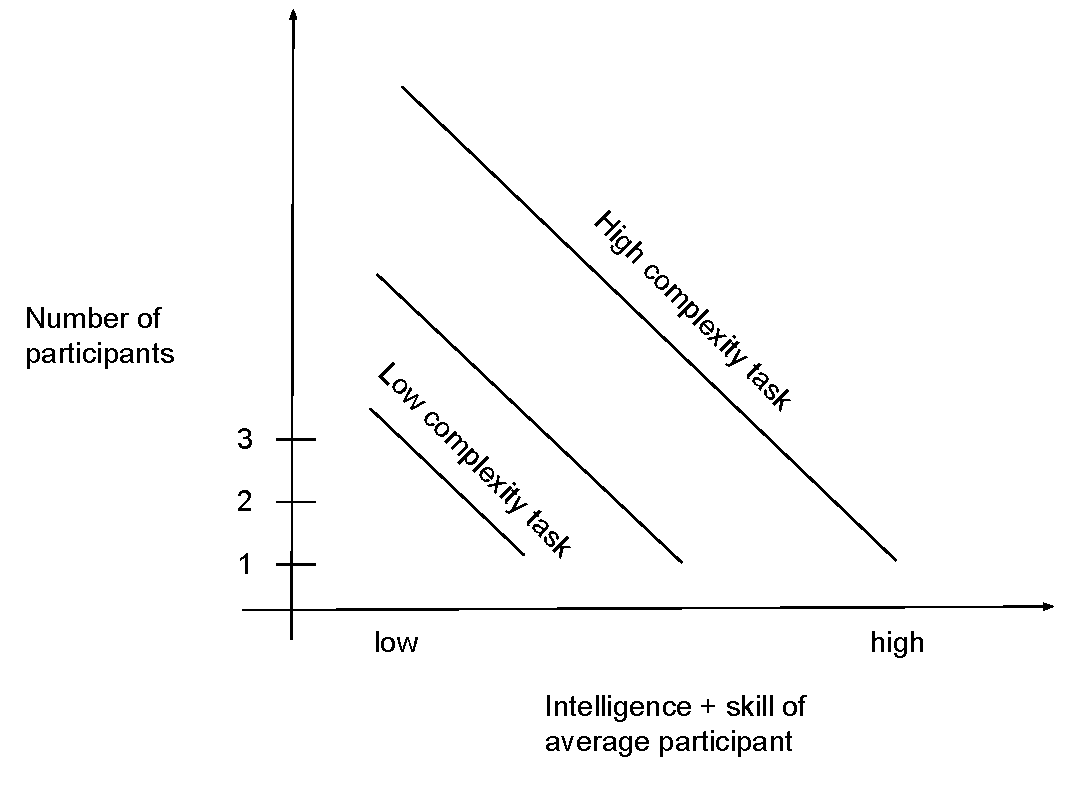
\includegraphics[width=0.8\textwidth]{images/people-per-task-for-skill-level.pdf}
\caption{A task that one smart person can do might take two dumb people. This concept applies to any task size and any population of workers. In this diagram three levels of task complexity are shown. As task complexity increases, the size of the team needs to grow. The growth may be less if the team members are brilliant. Those brilliant people cost more and there are fewer of them available.}
\label{fig:complexity-and-size}
\end{figure}


\subsection*{Automation of Processes}

The role of automation is to make interactions more predictable, faster, and to handle more of them. Automation does not eliminate bureaucracy; automation obfuscates the subjective decisions and limits the ability to negotiate with decision makers.

% https://graphthinking.blogspot.com/2019/07/bureaucracy-is-social-process-executed.html
There are benefits to automation, and automation can be implemented to minimize harm to bureaucratic subjects.  Automated systems can be made more transparent by including documentation about what is happening, why, and what's next.
\marginpar{[Tag] Actionable advice}
This helps both bureaucrats and subjects identify when assumptions made in the automation are incorrect. 


There are indicators of when to transition a human-based bureaucratic process to a more automated approach:
% https://graphthinking.blogspot.com/2019/07/cost-of-creating-and-supporting.html
\footnote{\href{https://xkcd.com/1319/}{https://xkcd.com/1319/} and \href{https://xkcd.com/1205/}{https://xkcd.com/1205/}}
\begin{itemize}
    \item The process to be automated is stable.
    \item The expected lifespan for the process -- how long the process will be needed -- is much longer than the time to implement the automation.
\item The process logic relies on objective evaluation criteria.  
\item The process is frequent.
\item The cost of automating (both the initial creation cost as well as the maintenance cost) represents a savings over the manual implementation.
\end{itemize}


\subsection*{Market-based Approach}
% https://graphthinking.blogspot.com/2017/09/market-friction-and-bureaucratic.html

There is an alternative to bureaucracy that features decentralized approach to complex tasks and avoids reliance on consensus: \href{https://en.wikipedia.org/wiki/Market_(economics)}{markets}.

An over-simplified definition\footnote{\href{http://www.investopedia.com/terms/m/market.asp}{http://www.investopedia.com/terms/m/market.asp}} is ``A market is a medium that allows buyers and sellers of a specific good or service to interact in order to facilitate an exchange." 
In practice, there is market friction: ``trading is always associated with certain costs or restraints."
\footnote{\href{http://www.investopedia.com/terms/f/frictionlessmarket.asp}{Frictionless market};
and \href{https://insight.kellogg.northwestern.edu/article/adding_friction_to_the_market}{Adding friction to the market}.}

The sources of friction in a market include
\begin{itemize}
    \item commissions on trades
    \item taxes (needed to fund contract enforcement organizations)
    \item uncertainty in hiring
    \item constraints on firing labor
    \item search cost in exploring the available opportunities
    \item risk uncertainty
    \item cost of creating contracts
    \item cost of insurance
\end{itemize}
Market friction and bureaucratic inefficiency are similar. \footnote{  \href{http://www.economist.com/node/17730360}{Why do firms exist?} and \href{https://en.wikipedia.org/wiki/The_Nature_of_the_Firm}{The Nature of the Firm}.}

Complex tasks at a societal scale range from manufacturing advanced computer chips, to creating and distributing critical medicine, to immigration and border enforcement. 
If a society wants to accomplish a complex task involving multiple people, then coordination of effort is required. The coordination can be explicit (in the form of a bureaucracy) or implicit (via a market).  Bureaucracy is one response to the complexity of a problem being solved.


\ \\

Regardless of whether a bureaucratic or market-based approach is used, 
% https://graphthinking.blogspot.com/2017/09/market-friction-and-bureaucratic.html
distributed knowledge and distributed decision making are hindered by aspects like
%\begin{itemize}
limited bandwidth between people participating in the coordination,
non-zero latency of information between people,
the cost of getting data,
and
the cost of analysis of data.
%\end{itemize}
Due to these factors, decisions that are suboptimal get made. See  %section~\ref{sec:dilemma-trilemma} 
the discussion of 
\hyperref[sec:dilemma-trilemma]{dilemmas}
for specific examples.

\ \\

The objective and quantified concept of money creates accountability that distinguishes commercial businesses from bureaucracy. Money as a metric is mutual to all participants within the business and money is in common with external stakeholders. 

Commercial businesses have employees who make subjective decisions and enforce policies, but unlike bureaucracy in business there is a common metric for feedback -- money. This distinction between business and bureaucracy is not sharp since the feedback mechanism is not perfectly applicable to all members of a business. Being an effective commercial bureaucrat may rely on the success of other employees rather than a direct interaction with customers.

Companies generally try to create profit. 
Bureaucracies like prisons, schools, hospitals, governments, and militaries all consume and spend money, but money isn't the goal. When faced with a decision, decisions are not guided by which will generate more profit. \cite{2012_Wilson}

\subsection*{Adhocracy}
% https://graphthinking.blogspot.com/2017/09/complex-tasks-necessitate-bureaucracies.html

Suppose I have a team of diverse experts assembled to tackle a complex challenge.
\footnote{\href{https://en.wikipedia.org/wiki/Adhocracy}{Adhocracy}}
While this may be sufficient for short duration tasks, if the challenge lasts more than a day or two there will be new issues beyond the original challenge:

\begin{itemize}
    \item Who pays the salary for this labor?
    \item Who calculates the payroll?
    \item Who pays the rent for facilities used by the team?
    \item Who does the maintenance on the facilities and equipment used?
    \item Who cleans the facility?
    \item Does risk incurred mean insurance is needed?
\end{itemize}
To address these questions that are out-of-scope for the complex challenge, you can either use a market-based approach or build a bureaucracy. 

\subsection*{Consensus Algorithms}

In the description of a \hyperref[sec:single-decider]{single decider}
%section~\ref{sec:single-decider} 
the solution was centralization of decision making and knowledge. Another approach to distributed decision making is to use consensus algorithms like \href{https://en.wikipedia.org/wiki/Paxos_(computer_science)}{Paxos} and \href{https://en.wikipedia.org/wiki/Raft_(algorithm)}{Raft}\footnote{For a tutorial on Raft see \href{https://raft.github.io/}{https://raft.github.io/}}.


\subsection*{Elected Representatives}
Governments are composed of politicians and bureaucrats. (Government isn't the only place bureaucrats appear, but for this section we'll focus on government.)

Political representatives are an easier to understand concept because it's just one person acting in that behalf of other people, and people get a vote in who that representative is.
In contrast, the emergent behavior of bureaucracy is more difficult to understand: many people are involved, and subjects of bureaucracy do not appoint the bureaucrats. 

% why not make the entire system out of politicians?
Suppose that instead of a bureaucracy all members of an organization charged with managing shared resources were elected rather than being selected for their technical skills. In this thought experiment we are eliminating one of Weber's characteristics of bureaucracy -- competence for job appointments. 

In the United States there are bureaucratic positions that feature a mix of election versus appointment. For example, the method of selecting judges varies widely by state \footnote{\href{https://ballotpedia.org/Judicial_selection_in_the_states}{Ballotpedia's breakdown of Judicial Selection by State in the USA}.}. In a 2017 survey, 63\% of more than 1000 judges favored appointment over being elected. \footnote{\href{https://www.judges.org/news-and-info/the-age-old-question-should-judges-be-appointed-or-elected-heres-what-you-said/}{2017 survey} and \href{https://www.judges.org/wp-content/uploads/2020/03/Q1_Text.pdf}{comments}}
% fascinating set of survey results:
% https://www.judges.org/news-and-info/five-years-of-question-of-the-month/

Attorney Generals in the United States similarly a selected by election and appointment.
\footnote{\href{https://ballotpedia.org/Attorney_General_office_comparison}{Ballotpedia's breakdown of Attorney General offices}.} Positions that benefit from expertise (e.g., Attorney Generals, Coroner) sometimes lack minimum qualifications when selected by election. Having an informed electorate capable of selecting competing candidates is challenging the more positions there are to vote on.

\subsection*{Small Organizations}

Suppose you try to limit bureaucracy by imposing that teams or organizations be small.

Given three people in a team, options are
\begin{itemize}
    \item split the labor among the participants; each has the same workload and same tasks. Consensus decision making; no exploitation of unique skills.
    \item split the labor by specialization; each becomes dependent on the other. Specialization enabled by scale can improve effectiveness but also incurs lobbying which decreases effectiveness 
    \item make one the manager to oversee the other two -- hierarchy. This is a specific form of specialization where one person is not directly involved in the labor.
\end{itemize}


\subsection*{Defending against Malicious Participants}

Suppose that you are part of an organization that doesn't have oversight processes for finances and the resources your organization is responsible for. A small percentage of the population, say 0.1\%, will take advantage of the lack oversight for their own gain. Those malicious actors can be either subjects of bureaucracy or bureaucrats within the organization. \href{https://en.wikipedia.org/wiki/Bruce_Schneier}{Bruce Schneier} calls these people defectors \cite{2012_Schneier}.

Similarly, suppose a small percentage of the population, say 0.1\%, is stupid and makes mistakes. Without a review process, these mistakes will negatively impact your organization's finances and the resources your organization manages. Preventing, detecting, and correcting mistakes can be costly investments. 

If you think bureaucracy sucks and it should be removed or replaced, then the parable of Chesterton's fence applies. 
\begin{quote}
There exists ... a fence or gate erected across a road. The more modern type of reformer goes gaily up to it and says, “I don’t see the use of this; let us clear it away.” To which the more intelligent type of reformer will do well to answer: “If you don’t see the use of it, I certainly won’t let you clear it away. Go away and think. Then, when you can come back and tell me that you do see the use of it, I may allow you to destroy it.\footnote{``The Thing'' (1929) Chesterton, in the chapter, ``The Drift from Domesticity''; \href{https://www.chesterton.org/taking-a-fence-down/}{https://www.chesterton.org/taking-a-fence-down/}}
\end{quote}
You need to understand the historical progression of each process that your organization relies on so that you understand why bureaucracy exists.

